\chapter{HSNA Process and Network Modeling}

% Social historians' goal is to characterize socio-economic phenomena and their dynamics on a restricted period and place of interest, and see how individual people of that time lived through them. For this, they rely on historical documents such as conversational letters, census, marriage acts etc. They usually extract qualitative and quantitative information from an identified corpus of documents, to then make quantitative conclusions on interesting socio-economic patterns. This can range from the distribution of jobs and social status, the migratory flux, to the structure of families in a given society. For this, historians can follow a Social Network Analysis (SNA) or more precisely a Historical Social Network Analysis (HSNA) approach. HSNA is a method---sometimes referred as a paradigm---which consists in modeling the social relationships between a set of entities---usually individuals---into a network, using the information from the historical documents. Very often, historians model the persons mentioned in the text as the nodes of the network, who are connected two by two by links modeling social relationships, such as friendships and family ties.
% However, textual sources can be rich in information and can refer to complex relationships involving more than two persons at the same time. Persons can also have different implications or roles as social relationships are often non symmetrical.
% For example, there have been several studies on business documents concerning financial transactions. These documents often involve more than two persons, who can have very different roles. Usually this type of document refers to sellers and buyers, but can also indicate other persons such as a guarantor, and/or some kind of notary. These complex relationships are hard to model into simple person-to-person networks.
% Furthermore, textual sources almost always contain extra information in regard of the event they refer to like the time, location, and other such as the type and amount of the transaction. It can also contain extra information about the persons such as their job, family and sex.
% It is clear that such information-rich data is difficult to model as person-to-person simple network. Even if more complex models have been proposed in the literature, such as dynamic or bipartite networks, simple networks are still the norm. In this paper, we first describe the social historians work process when they follow an HSNA, starting from the textual sources acquisition to the analysis and visualization of the network, and we identify potential fallback at each steps.
% Then, after describing the most used network models in HSNA, we formalize a network model which models well the majority of historical sources we encountered in all their complexity: \model. We give real world example on how this model has been used to follow HSNA pipelines, from data preparation to visual analysis using a visual query system. From these examples, we identify 3 properties of this model compared to simple networks: non-duplication of information, no ambiguity, and concordance of the original sources.

Tools for social network visualization tend to ignore the context in which the networks are produced, where they come from, and the workflow that led from their origin (e.g., documents, polls, interviews, web scraping) to their network form.
Yet, practitioners of social history needs to generate many networks from the same documents/sources to visualize and analyze them.
% and need to maintain the provenance from documents to analyzes and back.
% In this article, we explain why and how effective tools for supporting Historical Social Network Analysis~\cite{wetherell_historical_1998} (HSNA) should model social networks in multiple steps to support three essential principles: \emph{traceability}, connection to \emph{reality}, and \emph{simplicity}.
In this article, after describing and characterizing the workflow of Historical Social Network Analysis~\cite{wetherellHistoricalSocialNetwork1998} (HSNA) from our collaborations with social historians, we explain why and how effective tools for supporting this process should model social networks in multiple steps to support three essential principles: \emph{traceability}, connection to \emph{reality}, and \emph{simplicity}.

Social historians' goal is to characterize socio-economic phenomena and their dynamics in a restricted period and place of interest, and see how individual people of that time lived through those changes.
For this, they rely on historical documents such as conversational letters, censuses, and marriage acts.
They usually extract qualitative and quantitative information from an identified corpus of documents, to then make conclusions on interesting socio-economic topics such as migrations, business dynamics, education, and kinship.
For doing this, historians can apply Social Network Analysis (SNA), a method---sometimes referred to as a paradigm---which consists in modeling the social relationships between a set of entities---usually individuals---into a network.
Much work has been done to adapt SNA to the context of historical document exploitation, and although several approaches coexist they can be brought together under the banner of Historical Social Network Analysis~\cite{wetherellHistoricalSocialNetwork1998} (HSNA) or Historical Network Research~\cite{kerschbaumerPowerNetworksProspects2015} (HNR).
When following an HSNA, historians collect documents, annotate them, and construct a network from the annotations that they finally analyze and visualize to validate or find new hypotheses.
Unfortunately, the process is often linear and it is common that, when visualizing their network, historians spot errors and inconsistencies in the annotations that they could have fixed if the process was iterative.

Moreover, historical documents are often complex and the annotation and modeling process can be done in many different ways.
Several network models have been proposed ranging from simple and specific ones like co-occurrence networks to more general and complex ones such as multilayer networks and knowledge graphs.
Simple models allow answering specific questions and are easy to manipulate but are often too simplistic and may distort the information contained in the documents.
Moreover, they often break the traceability from the analysis to the original documents, making the communication of findings less reproducible and the process of cleaning the annotations complicated.
Indeed, errors and mismatches often occur in the annotation process, for example, due to entity disambiguation problems.
On the contrary, too complex models are complicated to visualize and analyze, and historians do not always have the tools to create them properly.
This paper proposes to model historical datasets as \modelplural, where both persons and documents are modeled as nodes with attributes.
While this model is simple enough for creation and inspection, it allows tracing back the entities of the network to the original sources for a continuous annotation process and still accurately models the social relationships mentioned in the documents.
Historians can therefore use this model to simultaneously find errors and inconsistencies in their annotation process---allowing them easier back and forth between the annotation and analysis steps---while starting a first analysis and exploration of the data to answer their sociological questions.
The traceability to the original sources also make the communications of findings more replicable and transparent.


% \jdf{Explain why the process is important to improve the analysis and more specifically the visualization}
% \jdf{Modeling the corpus vs.\ modeling the networks}
% \jdf{Modeling as a graph database allows expressing concepts at the right level of abstraction and can be handled interactively with novel tools (ours and others)}
% \jdf{Mention Scale: the problems are already there for small models that are typical, large models will come later}


% Very often, historians model the persons mentioned in the text as the nodes of the network, who are connected two by two by links modeling social relationships, such as friendships and family ties.
% However, historical documents are often rich in information and can refer to complex relationships involving more than two persons at the same time. Persons can also have different implications or roles in the documents, and relationships are often non symmetrical~\cite{lemercier_analyse_2005}.
% For example, there have been several studies on business documents concerning financial transactions~\cite{rossi_exploration_2014, crailsheimSpanishConnectionFrench2016}. These documents often involve more than two persons, who can have  different roles; this type of documents refer to sellers and buyers, but can also indicate other roles such as a guarantor, witness, or notary. These complex relationships are hard to model into simple person-to-person networks.
% Furthermore, textual sources almost always contain extra information in regard of the event they refer to like the date and time, location, and other such as the type and amount of the transactions. It can also contain extra information about the persons such as their job, family, and gender.
% It is clear that such information-rich data is difficultly modeled as a simple person-to-person network. Yet, even if more complex models have been proposed in the literature such as dynamic and bipartite networks, simple networks are still the most widespread model supported by popular tools.
% Moreover, a large number of HSNA studies focus on reporting network analysis results, but rarely give details on the encoding, annotation, and network modeling process even though these are primordial steps which influence greatly the final results. Therefore, it can be difficult for readers to trace back the analysis to the original documents, and can pose replicability problems \cite{baker_1500_2016}. For these reasons, network models that can more faithfully represent the complex reality of the documents while allowing traceability to the sources and are easy enough to manipulate are needed.
% In this paper, we first describe the HSNA work process that we have observed from the literature and collaborations, starting from the textual sources acquisition to the analysis and visualization of the network, and we identify potential issues related to analysis for each step.
% Then, after describing the most used network models in HSNA, we formalize a network model which satisfies \textit{reality} and \textit{traceability} properties, and
% which models well the majority of historical sources we encountered with their complexity: the \model. We give real world examples on how this model has been used to follow HSNA pipelines, from data preparation to visual analysis using a visual query system. From these examples, we identify three problems which arise when doing a network projection but not when using \modelplural: no loss of information, no duplication, and no distortion.

\section{Related Work}

Since we already elaborated on the related work of SNA, HNR, network modeling and social network visualization in \autoref{ch:related-work}, we only discuss in this section the related work concerning historians' workflow and methodology descriptions.

The essence of the historical discipline is based on a critical approach of sources and involves considering peers' work.
Traditional approaches of history often focus on the construction of a narrative, without necessarily adopting a systematic and problematized approach to the exploitation of original sources.
Social history and the ``Annales School'' proposed a new approach to history, by trying to describe and characterize socio-economic phenomena of the past by rigorously extracting information from historical documents and making conclusions from them.

With similar aims, Glaser and Strauss developed the ``Grounded Theory'' \cite{glaserDiscoveryGroundedTheory2010} as a methodology for the humanities to build hypotheses and theories by solely studying and categorizing real-world observations, without starting from prior knowledge and predefined categories.
Later on in the 1960s, quantitative methods started to be used in history, providing statistical and later computer-supported tools to aid historians in grounding their analysis in mathematical models and results.
Unfortunately, the lack of methodology and understanding between the two worlds led to many criticisms by historians pointing to using wrong metrics, simplifying categories, and disconnections between the original documents and analysis \cite{karila-cohenNouvellesCuisinesHistoire2018, lemercierBackSourcesPracticing2021}.
Quantitative history has been showed to be useful when used properly and when not focusing only on numbers, and several books have been published on how to efficiently use statistical methods such as summarizations, hairballs correlations, statistical distributions, statistical testing, time series etc. \cite{hudsonHistoryNumbersIntroduction2016, lemercierQuantitativeMethodsHumanities2019}.
Similarly, the use of HNR for historical purposes increased in the recent years, and a lot or resources exist on how to use network methods and measures for historical research \cite{lemercier12FormalNetwork2015, kerschbaumerPowerNetworksProspects2015}.

However, few work has been done on describing and formalizing the process before the analysis part for a quantitative and network research workflow.
Indeed, if it is central to know how to manipulate statistical and network concepts and methods when following this kind of methodology, it is as important if not even more to follow a correct and rigorous workflow to generate the data we plan to analyze beforehand.
The process to generate a clean quantitative or network dataset from historical sources is difficult and requires several data acquisition, annotation and cleaning steps.
Social analysts are not always trained on how to do these steps effectivity, which can lead to errors, inconsistencies, and mismatches between the chosen data models and the historical questions \cite{alkadi2022}.
Karila-Cohen and al.\ provide some advices on how to annotate historical documents in the aim of using quantitative methods \cite{karila-cohenNouvellesCuisinesHistoire2018} and prone that the annotation and analytical processes should not be dispatched between several persons, as both usually influence each other.
Dufournaud describes her workflow in depth when studying the socio-economic status of women in France in the 16th and 17th centuries, which she splits into three steps: \textit{data collection}, \textit{data processing}, and \textit{data analysis}~\cite{dufournaudCommentRendreVisible2018}.
She provides the tools and methodology she used to annotate her data, providing transparency on her historical analysis and methodological resources.
Cristofoli discusses the network modeling problem when following an HSNA and highlights the fact that the same historical documents can be modeled in different ways \cite{cristofoliAuxSourcesGrands2008}.
Historians should be aware of this and chose a network model which fits their analytical goals.


%HSNA, which can be seen as a sub-component of quantitative history has been criticized for similar reasons \cite{lemercier12FormalNetwork2015}.
%Still, the usage of networks for historical analysis provided some interesting results and classical works~\cite{padgettRobustActionRise1993}, meaning that a clearer and more rigorous methodology with simple tools grounded in the historian workflow and sources could improve the methods of the field.


\section{Historical Social Network Analysis Workflow}

From the literature and discussions with historians' collaborators, we propose an HSNA workflow divided into 5 steps: \textit{textual sources acquisition}, \textit{digitization}, \textit{annotation}, \textit{network creation}, and finally \textit{visualization and analysis}.
The workflow is presented in \autoref{fig:process} along potential and recurrent pitfalls.

\begin{figure}
%    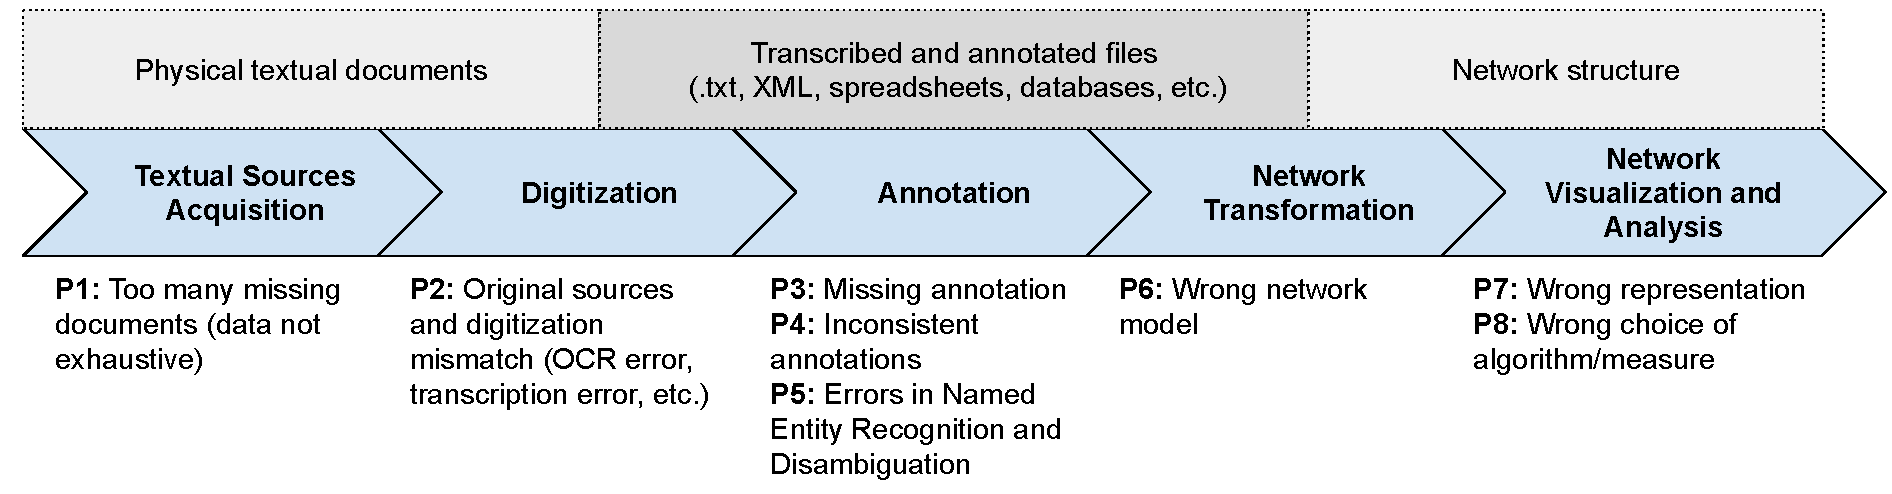
\includegraphics[origin=c, width=\textwidth]{static/figures/HSNAProcess/OriginalPaperFigures/Process5.pdf}
    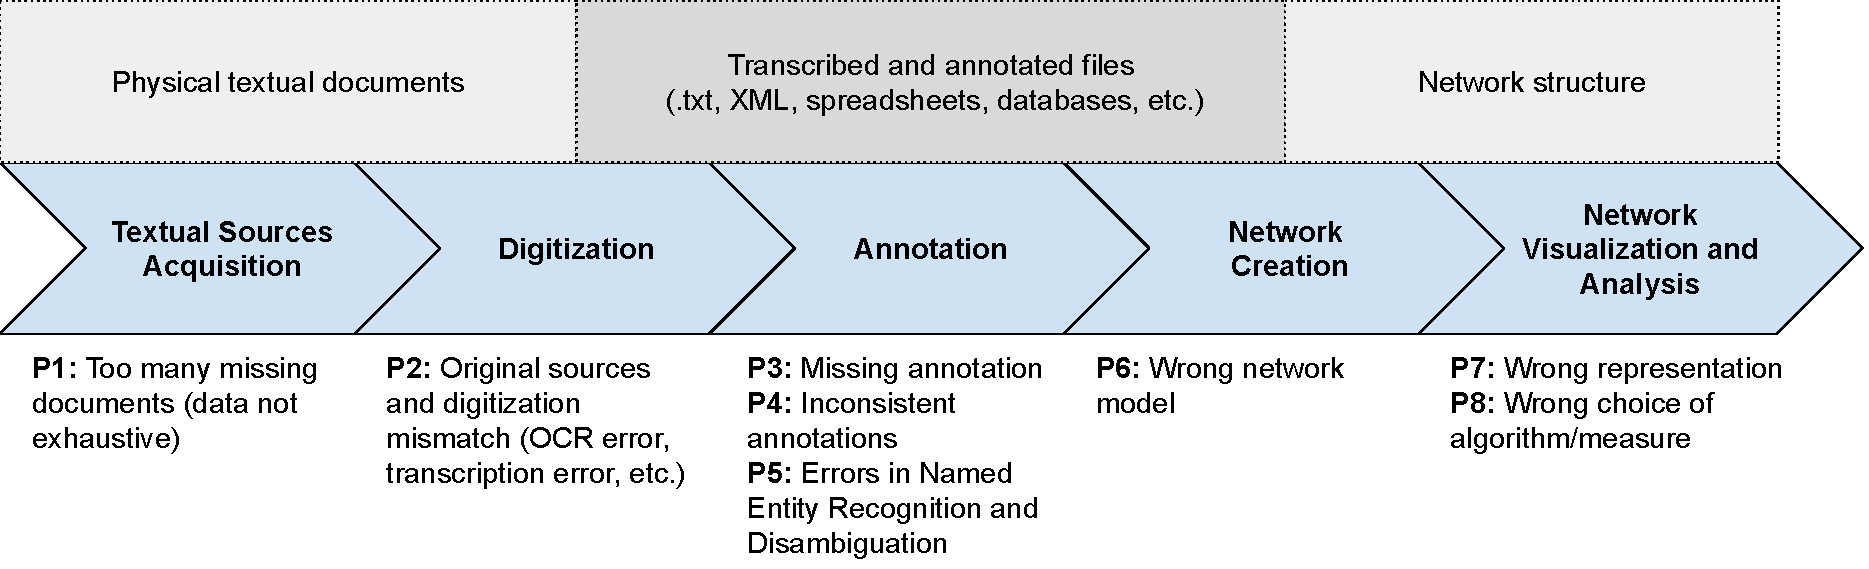
\includegraphics[origin=c, width=\textwidth]{static/figures/HSNAProcess/process.pdf}
 \caption{HSNA workflow split in five steps: textual sources acquisition, digitization, annotation, network creation, network visualization and analysis. We list potential pitfalls for each step.}
 \label{fig:process}
\end{figure}

% When following an HSNA, historians' goals is to characterize structural and individual socio-economic patterns between actors of a given period and place. For this, they try to model with a network real world social relationships and interactions between actors, that they extract from historical documents. By characterizing the structure of the network using visualization and analysis techniques, they can conclude on high level sociological conclusions \cite{wetherell_historical_1998}.

% This process is not straightforward, and has not been discussed a lot in the HSNA community. Dufournaud describes her workflow when studying socio-economic status of women in France in the 16th and 17th centuries, that she split in three steps: \textit{data collection}, \textit{data processing}, and \textit{data analysis} \cite{dufournaud2018comment}. From the literature and discussions with historians collaborators we propose an HSNA workflow description split in 5 steps: \textit{textual sources acquisition}, \textit{digitization}, \textit{annotation}, \textit{network creation} and finally \textit{visualization and analysis}. The workflow is presented in \autoref{fig:process} along recurrent potential issues which can arise.


%\noindent\textbf{Textual Sources Acquisition}
\subsection{Textual Sources Acquisition}
Historians' first step is gathering a set of textual historical documents mentioning people with whom they will have social ties.
For this, they usually take documents from a specific source---such as a folder from a national or local archive---and restrict them to a period and place that they want to study.
They also often restrict themselves to one document type---such as marriage or notary acts---to focus the analysis on one or few types of social relationships that they want to understand in depth.
However, one rule of the historian's method is to crosscheck from multiple sources, so an initial corpus is often extended with another set of related sources.
Once they restricted their search to a set of documents, a time, and a geographic area, they try to exhaustively find all the documents matching the desired properties, as \textbf{missing documents can result in uncertainty in the network structure and therefore the sociological conclusions (P1)}.

\subsection{Digitization}
%\noindent\textbf{Digitization}
Digitization consists in converting the sources into a digital format.
% \textcolor{green}{For modern history where the documents have been produced digitally or scanned and digitized through optical character recognition (OCR), this step can be skipped. For modern documents, digitization is now almost always done as it allows to tremendously ease the storage, indexation, and annotations of the documents} \textcolor{red}{
This step can be skipped for the most recent periods where many documents have been produced digitally or can be scanned and well digitized through optical character recognition (OCR), allowing to tremendously ease the storage, indexation, and annotation of the documents.
%, and facilitates the creation of a network object afterwards.
% is the only accessory step of the process, as everything can in theory be done without a computer,
However, before mid 20th century, most historical primary sources are stored in archives in paper format and need human work to be digitized.
% Digitization can be done by hand or with the help of Optical Character Recognition (OCR) tools.
\textbf{Mismatches between the original documents and the transcription can occur for old and recent documents (P2)}.
However, if OCR tools are more and more efficient in English and highly used languages, historians can work with old documents written in old or extinguished languages and with atypical writings (e.g., Fraktur handwriting and typefaces for German in the early 20th century).
Therefore, OCR tools are often unusable in social history and digitization remains an expensive and sometimes highly skilled process.

\subsection{Annotation}
%\noindent\textbf{Annotation}
Annotation is the process of finding and extracting useful information from the documents concerning the persons, their social ties, and any useful information for the historian.
This extra information can concern the persons (their age, profession, sex, ethnicity, etc.) and their social relationships (type, date, place).
It encompasses named-entity recognition (NER) as well as their resolution.
Historians also sometimes annotate information on other entities mentioned in the documents, such as art objects or administrative entities.
Usually, historians have a first idea of what they want to annotate in the data as they already explored the documents beforehand and have knowledge of their subject of study, with hypotheses they want to explore.
It is however common they can change their mind through the annotation process, by reflecting on what they found in the documents.
Unfortunately, this can produce \textbf{missing annotations (P3)} and \textbf{inconsistent annotations (P4)} at the end of the process if annotators are not careful.
This task can also be challenging and the choice of annotations has an impact on the final network.
Historians also face ambiguity in the process, as several persons and entities (like cities) can have the same name (homonyms), refer to a place name that has disappeared (street name or city), or to an ambiguous person (e.g., John Doe).
They, therefore, have to follow a NER and resolution/disambiguation process to identify entities in the sources and disambiguate them across several documents.
Entity resolution has always been a problem in social history---as it is more generally in text analysis, where typical groundwork consists in crossing information about the same entities from different heterogeneous sources.
However, errors in the disambiguation process can lead to important distortions in the final network structure and properties \cite{diesnerImpactEntityDisambiguation2015}, e.g, people connected to the wrong ``John Doe''.

Historians usually carry out this process manually but can also use automated methods and refine the results themselves later.
Unfortunately, \textbf{errors are common in this step as automated methods do not provide perfect accuracy, nor doing it manually given the lack of global information (P5)}.

The Text Encoding Initiative (TEI)~\cite{TEI} is an XML vocabulary and a set of guidelines typically used to encode and annotate documents, and the events happening in these documents (unclear parts, gaps, mistakes, etc.).
It is also used for historical texts and to generate social networks~\cite{dufournaudComparaisonOutilsPour2006, vistorian_mini_questionnaires}.
Unfortunately, the guidelines are not meant to define a canonical annotation and different persons can interpret the guidelines in different ways, leading again to inconsistent annotations of corpora (P4) and to errors or distortions in social networks derived from these annotations.
% Several softwares can be used for annotation and are usually stored in markups formats such as XML .

\subsection{Network Creation}
Historians construct a network from the annotations of the documents.
Usually, all persons mentioned are annotated and will be transformed into network nodes (vertices).
Additional information such as their age, profession, and gender can be stored as node attributes.
How the network's links are created is not as trivial and can vary from project to project~\cite{alkadi2022}.
The most straightforward approach is to create a link between every pair of persons mentioned in one document, thus forming a clique motif.
This is a simplistic heuristic as social relationships can be quite complex, involving more than two persons who can have different roles in the relationship.
The choice of the network model has a major impact on the future analysis and \textbf{may add bias if chosen loosely (P6).}
More complex models have been proposed in the literature such as weighted, dynamic, bipartite, and layered networks. % We discuss them more in depth in \autoref{sec:modeling}.

% A more factual approach consists in differentiating the roles of the persons in the documents and modeling them as link types. For example, for marriage acts, the witnesses will be linked with the spouses with a \textit{witness} link, while the spouses will be linked together with a \textit{spouse} link. However, there are often several possible representations, as the social relationships include several people and are difficult to represent as pairwise ties. For example, witnesses can be linked to one, or both of the spouses depending on the analysis goals. If a priest is leading the ceremony, he could be linked to the spouses, or the spouses and the witnesses.
% Furthermore, for both examples, there is a loss of information concerning the precise events and we may not retrieve who was mentioned in the exact same documents from the network alone. For example, if someone marry twice, we may not know which marriage the witnesses are from.
% To counter these issues, some historians transform their sources into bipartite networks (also called 2-modes and affiliation networks), where the sources are also modeled as nodes and the links model the occurrences of a person in a document, with their roles.

\subsection{Network Analysis and Visualization}
%\noindent\textbf{Network Analysis and Visualization}

% Once historians constructed a network they are satisfied with, they start exploring and analyzing it with visualization and quantitative methods.
% There is traditionally two schools of thought in SNA : Structuralism and Ego studies \cite{eve_deux_2002}. Structuralists are interested in studying the global structure and properties of the network, and leverage those to make conclusions on real social phenomena.
% In contrary, sociologists following ego studies focus more on specific individuals, and try to model all their social interactions whatever the type to understand other sociological attributes such as their status, or certain behaviours. This approach is thus often using ego networks, multiplex relationships and dynamic networks.
% Most HSNA studies usually involve concepts and methods from these two approaches \cite{cristofoli_aux_2008}, trying to make structural conclusions on how an organization operates while observing specific individuals in all their complexity.
% During the analysis, historians use visualization tools to gain a better understanding of the network's structure. It allows them to explore the network and detect interesting patterns rapidly. Most widely used tools are Pajek and Gephi, which also provide algorithms for the analysis, such as for community detection or structural analysis.
Once historians have constructed a satisfactory network, they start exploring and analyzing it with visualization and quantitative methods.
The final goal of HSNA is to find interesting patterns and link them to social concepts to gain high-level socio-historical insights \cite{freeman_development_2004, wetherellHistoricalSocialNetwork1998}.
Usually, historians start to visualize their network to visually confirm information they know, then to potentially gain new insight with exploration.
Representations need to be chosen wisely given the network as lots of techniques and tools exist for social network visualization. \textbf{Some insight may be seen only with some specific visualization technique (P7)}.
To test or create a new hypothesis, historians typically rely on algorithms and network measures.
Lots of network measures have been developed like modularity, centrality and clustering coefficient that social scientists can leverage to make conclusions \cite{scottSocialNetworkAnalysis1988}.
Similarly, social scientists can use data mining algorithms to highlight interesting and potentially hidden structure in the network, e.g. by using clustering algorithms revealing group structures \cite{brandesModularityClustering2008}.
\textbf{However, they have to interpret the results carefully (P8)} as some algorithms act as black boxes and some measures are hard to interpret, with unclear sociological meaning (e.g., centrality).
Typically, particular patterns and measures values in the network could have different potential sociological meanings.
If we take as an example betweenness centrality which measures the number of time a node appear in the shortest path of every pair of existing nodes, individuals with high values usually highlight positions of power as they communicate with different groups.
However it can also be interpreted as a position of vulnerability in other contexts such as during periods of wars and repressions, as in the study of Polish social movements in the 20th century by Osa \cite{osaSolidarityContentionNetworks2003} where she shows persons with high betweenness centrality values are more targeted for repression in certain periods.
Social scientists therefore have to be careful when interpreting network measures, and take into account the globality of their sources when interpreting the network they constructed.


\section{Network modeling and analysis}\label{sec:modeling}

% \subsection{Quantitative History}

% Traditionally, historians try to tell a story about protagonists and socio-economic facts in a given society. This narrative approach of history have been criticized for its lack of traceability and the open interpretation of historical documents, which can introduce bias from the author.
% Social history and HSNA brought answers to this problem by bringing quantitative methods to enforce a narrative supported by data and statistical results. However, traditional HSNA studies describe globally their sources without precising the annotation and transformation process they followed. They don't mention how the network they study has been obtained from the sources. Yet, these steps are critical as they can deeply influence the results of the analysis \cite{lemercier_analyse_2005} \cite{cristofoli_aux_2008}. Indeed, historians have to make choices on what to annotate and what to model into the network. This often depends on what they want to demonstrate at the end.
% As these steps of the workflow are often not transparent, it can be difficult for the reader of an HSNA study to understand how does the network has been constructed, what it represents, and to trace back the network entities from the original sources \cite{dufournaud2018comment} \cite{dufournaud_recherche_2015}.

% Recently, Experimental Computer Science went through a replicability crisis, pointing out that a lot of results were not reproducible, since authors were not giving enough data or information for people to redo the same analysis. Reproducibility is though considered a condition for building scientific knowledge, and this discussion highlighted the fragility of a lot of experimental studies. Data shows that the natural and social sciences are also affected \cite{baker_1500_2016}.

% Usage of computer science in history can mitigate this problem, by providing methods and tools for historians to follow their analysis and providing traceability from their high level conclusions to the original documents.

% We argue one way of doing that is to use a network model which reflects well the \textbf{reality} of the social relationships mentioned in the documents, and are \textbf{traceable} to the original sources. We think network models which satisfy these two properties---\textbf{reality} and \textbf{traceability}---should always be constructed from the original sources as a basis for the analysis. Other network transformations can be applied afterwards to reveal specific patterns, but having a network which reflects well the reality of the documents is primordial for representing the sources as they are, and allowing to easily go back to them at any point in the analysis. Indeed, any transformation can be applied from a network representing well the sources. But applying modifications and transformations directly in the annotation process can bias the analysis and remove the possibility to follow other explorations and hypothesis in the future.

% Indeed, historians have to make choices on what to annotate and what to model into the network. This often depends on what they want to demonstrate at the end.
% As these steps of the workflow are often not transparent, it can be difficult for the reader of an HSNA study to understand how does the network has been constructed, what it represents, and to trace back the network entities from the original sources \cite{dufournaud2018comment} \cite{dufournaud_recherche_2015}.

% When transforming the information of the documents into a network, historians have to make choices on what to annotate and what to model into the network. As these steps of the workflow are often not transparent, it can be difficult for the reader of an HSNA study to understand how does the network has been constructed, what it represents, and to trace back the network entities from the original sources \cite{dufournaudCommentRendreVisible2018}. Also, too complicated models are harder to visualize and analyze. For these reasons, we argue that a good network model should reflects well the reality of the social relationships mentioned in the documents, is traceable to the original sources, and is simple enough to visualize and understand.
% We think network models which satisfy these three properties---\textbf{reality},  \textbf{traceability} and \textbf{simplicity}---should always be constructed from the original sources as a basis for the analysis.

Historians typically construct one or several networks from their annotated documents that they will visualize and analyze to validate or find new hypotheses.
As the processing steps of the workflow are often not transparent (digitization, annotation, network modeling), it can be difficult for the reader of an HSNA study to understand how the network has been constructed, what it represents, and to trace back the network entities to the original sources \cite{dufournaudCommentRendreVisible2018}.
Moreover, visualizing the network very often highlights errors and artifacts of the annotations, along with potential mismatches between the network model and the analysis goals.
Historians then have to correct or change their annotations, even though it is a very tedious and demanding process  to repeatedly switch back and forth between the network and the annotated documents.
Several network models make the task harder as they do not directly represent the documents, and it is thus difficult to relate a network entity to a specific document and annotation.
Therefore, we believe that more visual analytics tools should support social scientists in annotating and modeling their documents to make the HSNA process less linear by allowing easier back and forth between the annotation, modeling, and visualization steps.
Network models satisfying  \emph{traceability}, \emph{reality} and \emph{simplicity} properties would mitigate those problems by allowing to navigate more easily between the network and the documents while still modeling well the social relationships mentioned in the sources and being easy enough to visualize and manipulate for analytical and cleaning goals.
%the data and detect potential errors and inconsistencies.

\subsection{Network Models}

Currently, historians use various network models depending on their knowledge of network science, the content of their documents, the schema of their annotations, and the analysis they plan to make.
We describe here the most used network models in HSNA along with more recent ones:

\begin{itemize}[nosep,leftmargin=*]
    \item \textbf{Simple Networks~\cite{wetherellHistoricalSocialNetwork1998}:} According to their research hypotheses, historians select and merge document information to build a specific relationship between individuals. They analyze this simple network structure with SNA tools and produce network indicators and node-link visualizations. It is often difficult to connect the results to the original sources.
    \item \textbf{Co-occurrence networks \cite{sairioMethodologicalPracticalAspects2009}:}
    % rubio-mondejarWomenEntrepreneursFamily2022}: % , keekMovementPerspectivesCollective, bouletBatchKernelSOM2008
    Only the persons are represented as nodes, and two persons are connected with a link when they are mentioned in the same document (or section).
    This is a simple model and one of the first to have been used in SNA and HSNA. The major drawback of this model is that it does not take into account the diversity of social relationships, as every link is identical. It can work well when only one type of social relationship is studied like a friendship network \cite{morenoFoundationsSociometryIntroduction1941}. However, historical documents rarely mention only one type of relationship and this model is thereby very limiting for HSNA.
    \item \textbf{Multiplex Unipartite Networks \cite{eriksonMalfeasanceFoundationsGlobal2006}:} Only the persons are represented as nodes, and links model social ties between two persons. Links can have different types representing different types of social relationships. It allows to model more complex social relations where people can have various social ties e.g. as parent, friends, and business relationships. However very often several possible representations for the same data exist as projections are often applied to the original documents to get this type of model. One of the main drawbacks of this model is that it creates parallel edges that are hard to visualize.
    %, and very often several possible representations for the same data exist, especially for complex relationships. [jdf] true for the other network types
    \item \textbf{Bipartite (also called 2-mode) Networks
    \cite{hambergerScanningPatternsRelationship2014}
    % \cite{hamberger_scanning_2014, lippPetitionsSocialContext2001a, shafie_hypergraph_2017}
    :} Nodes can have two types: persons and documents in this network model. A link refers to a mention of a person in a document and can thus only occur between persons and documents nodes. Usually, links are not typed and only encode mentions.
    More recent analysis in HSNA encode the \emph{roles} of the persons in the documents as link types~\cite{cristofoli2018}. This network model is more aligned with the original sources and allows following an analysis through the original documents themselves and not through concepts. For example, the GEDCOM format introduces the concept of ``family'' that ties together a husband, spouse, and children with different link types.
    However, the concept of family can have different meaning across time and cultures, meaning that GEDCOM adds a conceptual layer instead of grounding the network to concrete traceable documents and events (e.g., no marriage but birth certificates).
    % In our model, a family tie would be replaced by different documents: the marriage certificate and  birth certificates, to ground the network to concrete traceable documents and events.
    \item \textbf{Multilayer Networks \cite{multilayer}: } in these networks, each node (vertex) is associated with a \emph{layer} $l$ and becomes a pair $(v, l)$, allowing to connect vertices inside a layer or between layers. These advanced networks have received attention from sociologists~\cite{CRNOVRSANIN201456} and historians~\cite{vanVugt_2017}, but they are complex. The meaning of a layer varies from one application to another; it can be time (years), type of documents, the origin of sources, etc. They, therefore, offer many (too many) options for modeling a corpus, and visualizing it, with no generic system to support historians for taming their high complexity.
    \item \textbf{Knowledge Graphs (KG)\cite{kgraphs}: } they represent knowledge as triples $(S, P, O)$ where $S$ is a \emph{subject}, $P$ is a \emph{predicate}, and $O$ is an \emph{object}. Everything is encoded with these triples using controlled vocabularies of predicates and rules known as \emph{ontologies}. KG is popular for encoding knowledge on the web, including historical knowledge. However, it is notoriously complex to encode documents using KG due to the complexity of the format and the wide choice of possible ontologies. Most historians are unable to understand KG and even less to use it for annotating a corpus. Since KG are generic, they need complex transformations to be visualized, with no generic system to support historians in taming  their high complexity.
\end{itemize}

\begin{figure}
    \centering % avoid the use of \begin{center}...\end{center} and use \centering instead (more compact)
    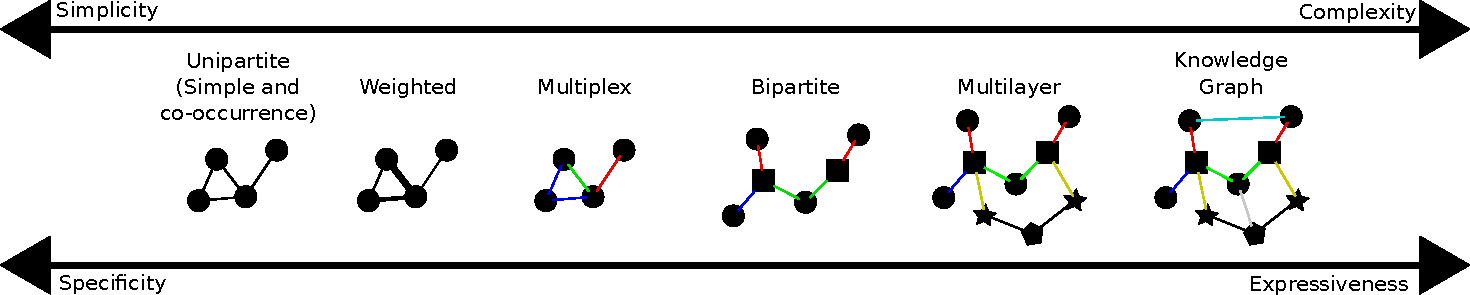
\includegraphics[width=\columnwidth]{static/figures/HSNAProcess/OriginalPaperFigures/models.pdf}
    \caption{Schematic representations of Different network models used for analyzing historical documents, ordered by complexity and expressiveness}
    \label{fig:network-models}
\end{figure}

\autoref{fig:network-models} shows a schematic representation of the different network models.
We can rank the models given two axes: simplicity/complexity and specificity/expressiveness.
Currently, historians mostly construct unipartite networks (simple, co-occurrence, and weighted) which are simple and allow them to answer specific questions.
However, those models do not capture all the complexity of the documents and social scientists may miss important patterns.
For example, modeling only co-occurrences of persons in documents remove the variety of social relationships these mentions can refer to \cite{lemercier12FormalNetwork2015}.
Several interpretations may coexist to explain why someone is central in the resulting network, which may be impossible to validate without encoding more information---such as the types of relationships---in the model.
Depending on the schema of the annotations, it may be impossible to create more complicated networks at this step without redoing the annotation process which is costly in time and resources.
On the contrary, too complicated models such as KG are difficult to create from the sources and are hard to visualize and analyze, especially for social scientists who are not trained in those kinds of formalisms.
Using this kind of model usually require learning complex query language to manipulate the data, such as the SPARQL language for KG\@.
Therefore, we argue that historians should aim to model a network that is simple enough to manipulate, can be traced back to the original sources, and model well the social reality of the documents---i.e. having those three properties: \textit{simplicity}, \textit{traceability}, and \textit{reality}.

\iffalse
Unipartite (co-occurrence and multiplex) networks are still the norm in the literature. However, we believe that if this type of model can be useful for SNA, they often bring distortion and ambiguity to historical datasets, which are complex. Cristofoli argues that using a bipartite network allows modeling the social relationships with a better alignment with the original sources and points to two drawbacks of using unipartite projections\cite{cristofoli_aux_2008}: the information about the specific events is lost, meaning that historians cannot make the connection between a link and the event/document it was created from. Furthermore, several projections exist for the same network, meaning that social scientists must choose which projection to use.
Moreover, historical sources typically contain extra information related to the persons and events mentioned. For example, it is not rare that a marriage act or a business contract mentions the jobs and the ethnicity of the persons mentioned. These types of documents also almost always refer to the date and location of the event, and sometimes more.
Traditionally, social scientists were not directly modeling this extra information into their network, which was considered a purely structural object. However, more modern studies try to incorporate this rich information directly into the network with more complex models such as dynamic and multivariate graphs. Abundant work has also been done in visual analytics to explore and analyze these more complex networks~\cite{refs}.
\fi

\subsection{Examples}\label{sec:examples}

We discussed with four experienced historians collaborators at different steps of their HNSA workflow about
their annotation process and how they wanted to model their network.
They all work on semi-structured historic documents, mentioning complex relationships.
We provide more details in the following:

\newcommand{\pascal}{\#1\xspace}
\newcommand{\nicole}{\#2\xspace}
\newcommand{\zacarias}{\#3\xspace}
\newcommand{\dana}{\#4\xspace}
\newcommand{\myindent}{~~} % ~\rule{1pt}{6pt}
\begin{enumerate}[nosep,leftmargin=*]
    \item Analysis of the social dynamics from \textbf{construction contracts in Italy in the 18\ts{th} century\cite{cristofoli2018, Rolla2018}.}
    %\textcolor{red}{PC: The corpus was created by N. Rolla through the exploitation of the manuscript registers of the \textit{Azienda generale fabbriche e fortificazioni} (State Archives of Turin)[REF : Rolla Nicoletta, 2018, "Mobilité et conflits. Travailler sur les chantiers de construction piémontais dans la première moitié du XVIIIe siècle" dans Andrea Caracausi et Marco Schnyder (eds.), Travail et mobilité en Europe (XVIe-XIXe siècles), Villeneuve d’Ascq, Presses universitaires du Septentrion (coll. Histoire et civilisations), p. 49‑72]. }
    The corpus is made of contracts for different types of constructions in the Piedmont area in Italy. People are mentioned under three different roles: \textit{Associates} who are in charge of the construction, \textit{Guarantors} who bring financial guaranty and \textit{Approvers}, who vouch for the guarantors. Documents contain information about the building site, the type and materials of constructions, and the origin of the people.
    \item Analysis of migrations from the \textbf{genealogy of a french family between the 17\ts{th}--20\ts{th} centuries} [unpublished work].
    The corpus is made of family trees referring to several document/event types: birth and death certificates, marriage acts, military records, and census reports.
    The roles are different for each event types, and consist in \textit{children, father, mother} for the birth events, \textit{deceased} for the death event, \textit{spouse} and \textit{witnesses} for the marriages, and \textit{family member} for the census events.
    \item Analysis of migrations from Spain to Argentina through the \textbf{marriage acts at Buenos Aires in the 17--19\ts{th} centuries ~\cite{moutoukias2016buenos, rueda1989matrimonios}.}
% \textcolor{red}{PC: The corpus was created by Z. Moutoukias \& C. Prieur through the digitization and annotation of a publication of the Buenos Aires Archives [REF: Jauregui Rueda, Carlos, Matrimonios de la catedral de Buenos Aires, 1747 – 1823, Buenos Aires, Fuentes Genealógicas e Históricas Argentinas, 1989]. }
    The corpus is made of summaries of marriage records that mention the spouses and the witnesses of the wedding.
    The origin, date of birth and parents names are specified for both spouses.
    % These parenting relationships are important for our collaborator, but do not refer to the same event as the marriage. Thus, we create another event node referencing the birth event, with \textit{father, mother}, \textit{child} as roles and the associated birth year and location as node attributes.
     \item Socio-political analysis of \textbf{migration of ethnic Germans from communist Romania to West Germany in the 20th century (ongoing work)~\cite{diminescu:hal-02556007}.}
     The corpus is made of administrative forms that mention persons requesting to migrate, along with the persons they want to join, and the administrative persons of the ministry in charge of the forms.
     The family members of the aspiring migrants are also mentioned in the forms, with their respective date of birth.
\end{enumerate}

We compare what would be the resulting networks for the three first examples (the example \dana is still in the phase of data acquisition) when modeling the data with the three most frequently used network models in HSNA: co-occurrence, multiplex unipartite, and bipartite networks.
We also encode important information from the document as network attributes.
We do this for one given document for each dataset.
The results are shown in \autoref{tab:models}.

As shown by Cristofoli \cite{cristofoliAuxSourcesGrands2008}, we can clearly see the co-occurrence model removes the complexity of the social relationships and only shows an abstract "proximity" between individuals.
Unipartite projections allow to produce meaningful networks which model well the diversity of relations that can link several people.
It especially models well simple relationships such as parenting ones as in example \nicole.
However, it produces distortions for more complex relationships involving more than two persons, as in example \pascal where people can either be mentioned as associates, guarantors and approbators in the documents.
Associates should probably be linked together with \textit{associate} links, but the \textit{guarantors} and \textit{approbators} relationships are more complex to model.
Approbators could be linked to the associates, the guarantors or both.
The three ways of modeling this type of relation makes sense, but can lead to very different network shapes and analysis results.
Historians thus have to decide on a transformation among several possibilities, which will probably distort the social reality of the relationships.

Moreover, projections adds ambiguity in retrospect of the original documents, as it becomes impossible to trace back one link to one specific documents, as the same link could potentially refer to several ones \cite{cristofoliAuxSourcesGrands2008}.

Finally, these examples show that when working with multivariate networks, using projections to create unipartite networks brings a duplication of information.
% brings problem which is not discussed in the literature which is the duplication of information.
Indeed, if a document mentions an information like a date that we model as an attribute, we can store it as a document node attribute using a bipatite model.
However, when projecting the network this information appears in the links as many times as there are persons mentioned in the document minus one and often more.
For example, in the example \pascal in \autoref{tab:models} the time is stored in $\sum_{i=1} ^{4} i = 10$ links in the co-occurrence model and in 9 links in the multiplex unipartite model while it is only stored once as a document node attribute in the bipartite model.
%For example, if a document mention five people, when creating a co-occurrence Network the time data will appear in the $\sum_{i=1} ^{4} i = 10$ links created.

\begin{table}
    \begin{tabular}{|m{4.4cm}|m{2.4cm}|m{2.4cm}|m{2.4cm}|}
        \hline Original Document & Co-occurrence & Unipartite representation & Bipartite \\
        \hline
        % \centering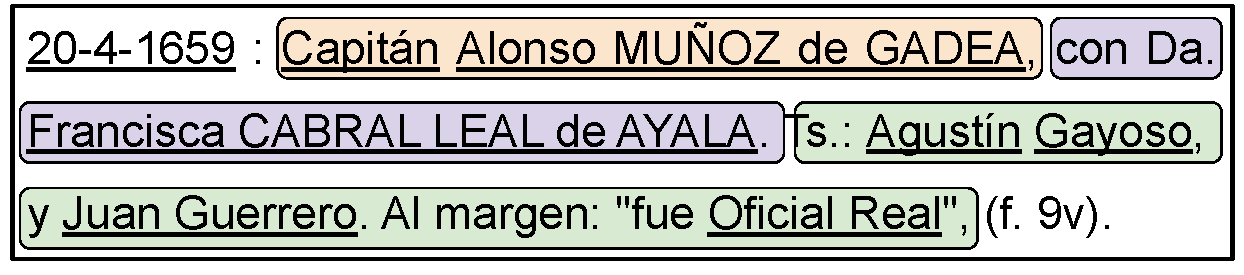
\includegraphics[scale=0.3]{OriginalPaperstatic/figures/HSNAProcess/OriginalPaperFigures/marriageDocumentnoParents}
        \tiny \underline{20-4-1659} : \colorbox{epoux}{\underline{Capitán} Alonso MUÑOZ de GADEA}, con Da. \colorbox{epouse}{Francisca CABRAL LEAL de AYALA}. Ts.: \colorbox{temoin}{Agustín Gayoso}, y \colorbox{temoin}{Juan Guerrero. Al margen: "\underline{fue Oficial Real}"}, (f. 9v). \linebreak
        \colorbox{epoux}{Husband} \colorbox{epouse}{Wife} \colorbox{temoin}{Witness}
        & \centering\simple & \centering\noParents & \bipartiteNoParents \\
        \hline \tiny \underline{1712}: Construction of a church in \underline{Torino}.
        Associates: \colorbox{associate}{Bellotto G, Bello P.M, Bello G.}
        Guarantor: \colorbox{guarantor}{ Astrano G.A.}
        Approbator: \colorbox{approbator}{Corte A.} \linebreak
        \colorbox{associate}{Associate} \colorbox{guarantor}{Guarantor} \colorbox{approbator}{Approbator}
        & \centering\simplePiemont & \centering\unipartitePiemont & \bipartitePiemont \\
        % \hline Le 7 octobre 1901, \colorbox{father}{François Marie Esnault} et \colorbox{mother}{Marie Julie Léopoldine Colson} ont déclaré la naissance de leur fille, nommée \colorbox{child}{Blanche Esnault} dans la commune de Saint-Maur-des-Fossés.uuu
        \hline \tiny Du \underline{dix-neuf fevrier mil huit cent quatre-vingt quatre}, à six heures du soir.
        Acte de naissance de \colorbox{child}{Dufournaud Alexis, enfant de sexe masculin} né le \underline{dix-neuf février}, à deux heures du soir au \underline{village de Grudet, commune de Saint} \underline{Symphorien}, des mariés \colorbox{father}{Dufournaud Alexis}, \colorbox{father}{cultivateur colon, âgé de trente ans}, et \colorbox{mother}{Marie Pardonnaud,} \colorbox{mother}{sans profession, agée de vingt-six ans}, demeurant au village de Grudet, dite commune de Saint-Symphorien. [...]
        \linebreak
        \colorbox{father}{Father} \colorbox{mother}{Mother} \colorbox{child}{Child}
        & \centering\birthSimple & \centering\birthUnipartite & \birthBipartite\\
        \hline
    \end{tabular}
    \caption{Resulting networks using different models produced by one document of the examples detailed in \autoref{sec:examples}: co-occurrence, unipartite and bipartite models. The first column shows the partial transcription of real documents. Colors represent annotations concerning the persons mentioned, their roles and attributes. Underline refer to information related to the events and which can be encoded as document/event attributes.
    H: Husband, W: wife, T: Witness, M: Marriage, $A_N$: Associate, G: Guarantor, Ap: Approbator, C: Construction, F: Father, M: Mother, C: Child.
    }\label{tab:models}
\end{table}


\subsection{Bipartite Multivariate Dynamic Social Network}

We argue that \modelplural verify the \textit{simple} \textit{traceability} and \textit{reality} principles and model well the majority of historical documents.
It has the following properties:
\begin{description}[nosep,leftmargin=2mm]
    \item[{Bipartite:}] There are \textbf{two types of nodes}, persons and documents (or events). An event, such as a marriage, is most of the time witnessed by a document, and we refer to them interchangeably as events and documents. Events considered in the network can be of the same sub-type, such as contracts, or of multiple subtypes, e.g. for genealogy: \emph{birth certificates}, \emph{death certificates}.
    \item[Links and Roles:] A link models the mention of a person in a document. \textbf{Each link has a type corresponding to the role of the person in the document}. For a marriage act, the roles include \emph{wife}, \emph{husband}, \emph{witness}. This is a key aspect of our model since it clarifies the relationship between the persons within an event. In contrast, Jigsaw~\cite{Stasko} does not consider the roles.
    \item[{Multivariate:}] Each entity of the model can have attributes, that give additional information. Person nodes are referenced by a key that reflects the disambiguation process. They can have general information (standardized name, gender, birth date). Documents are also identified by a key, e.g., an archive reference. The associated event can have a date, sometimes a location, and potentially other information. Links can also carry information to describe contextual properties (activity, residence, etc.).
    \item[{Geolocated:}] Events should have a location when it makes sense, ideally with the longitude and latitude.
    \item[{Dynamic:}] Events are always dated. We rely on this date since it encodes the social dynamics of the network.
\end{description}

One of the main benefits of this model is that the document nodes represent both the physical documents and the events the documents refer to.
For example, concerning marriage acts, the document nodes represent both the physical documents with their texts but also the marriage events with their characteristics modeled as attributes (time, location, etc.).
Therefore, social historians can use this model to store, process and clean their original documents and follow an analytical workflow with the same representation.
This model is \textit{simple} enough to manipulate and visualize for historians and allows tracing back every entity of the network to the documents according to the \textit{traceability} principle.
Still, the network preserves the \textit{reality} of the social relationships mentioned in the sources as no projection or transformation are applied.
%More precisely, Cristofoli demonstrates that bipartite networks ensure no distortion or ambiguity, unlike projected networks when modeling textual sources \cite{cristofoli_aux_2008}.


%Furthermore, when attributes are encoded, projected networks provoke a duplication of information related to the events. For example, the date of a marriage can be encoded in the document/event node with a bipartite network while the same information would have to be stored in several links when using a projection.

% We argue that the social relationships mentioned in historical documents are well modeled by bipartite networks, while preserving a connection between the network data and the original sources.
% Moreover, recent studies sometimes incorporate attribute information such as the time, location, and sometimes more.
% We therefore propose a document-oriented data model based on bipartite networks, and incorporating the time, location and any other information related to the persons and events. It has the following properties:
% We therefore propose a document-oriented data model for social networks, grounded on historical sources and persons, with the following properties:
% % unifying the models of PUCK and Jigsaw, with the following properties:

% This network model satisfy the \textit{reality}, \textit{traceability} and \textit{simplicity} properties. From the examples of \autoref{tab:models}, we leverage three properties of this model:
% From the examples of \autoref{tab:models}, we

\iffalse
We leverage three problems that arise when doing a projection that do not occur when using the proposed model:
\begin{enumerate}[nosep,leftmargin=*]
    \item \textbf{No information loss:} When projecting the original source into a person-to-person network, we cannot trace the original events links refer to. We know if pairs of persons have been in events together, but it become impossible to know which one. Moreover, we lose the fact that more than two persons appear in the same event together, as relationships become pairwise only.
    \item \textbf{No duplication:} When using document nodes, the information related to the events such as the time and location can be directly tied to those node, whereas the same information is duplicated in several links when projecting the data into an unipartite network.
    \item \textbf{No distorsion:} Most relationships referred in documents are complex and are complicated to model as pairwise relations. Creating a unipartite network often create some bias as several coexisting representations may exist. In contrary, bipartite network represent well the reality of the social relationships, as they model the data as it is written in the documents.
\end{enumerate}
\fi

\iffalse
\textcolor{red}{\emph{Quelques arguments si besoin a placer ici ou dans la discussion (je réalise que certains sont intégrés dans la discussion des modèles):\\
Un tel modelèle de bas niveau (réseau du corpus documentaire) permet :\\
- D'indexer rapidement un corpus documentaire (et de permettre de l'explorer facilement)
    - de rendre visible et de maitriser de manière opérationnelle la phase d’appariement des mentions d’individus observés dans les documents (si cette phase n'existait pas, le corpus serait composé d'étoiles non connectée, ca r ce qui fait la laison ce sont les identifications entre mentions d'individus)\\
    - donne la possibilité de reconstituer et de suivre les trajectoires des individus observés dans les documents : situer dans le temps et contextualiser la chronologie des relations entre les individus (et ainsi d’étudier la configuration relationnelle dans sa dynamique et sa multiplexité, et de repérer des profils et trajectoires relationnelles spécifiques).\\
    - Selon les besoins et la problématique, en combinant ébventuellement avec un filtrage des attributs, on pourra ainsi travailler directement sur le réseau 2-mode (requêtes) ou construire des projections contextuelles sur l’un de ces deux modes (individus ou documents) en produisant des réseaux uni-mode multiplexes, d'explorer et parcourir le corpus à l’aide de visualisations classiques en nœuds-lien ou via des visualisations alternatives matricielles (Valdivia et al. , 2020).\\
    - L’exploitation de ce réseau spécifique – multiplexe et dynamique – combine gestion et sélection de données, calcul de statistiques descriptives et construction d’indicateurs synthétiques, ainsi que la mobilisation des outils, mesures et procédures développés dans le cadre de l’analyse des réseaux.\\
    - La question de la visualisation pour l'exploration de ce type de réseau
    2 modes: Plus de sommets, moins de cliques "artificielles".
    Vue locale contextuelle du profil relationnel des individus.
    - En conclusion de la discussion, on peut poser la question du choix des documents et de l'importance de réfléchir à la façon dont le corpus forme un ensemble cohérent du point de vue de la recherche et de sa représentativité.
}
}
\fi

\section{Applications}

%% After constructing their network, historians can explore and analyze them using specifically designed visual analytics tools.
%Several tools have been designed for visualizing dynamic bipartite networks that can also be considered dynamic hypergraphs~\cite{valdivia_analyzing_2021, penaarayaHyperStorylinesInteractivelyUntangling2022}, but few incorporate attributes and complex interactions.
%We designed ComBiNet~\cite{pister2022visual} to explore and navigate through historical documents modeled as \modelplural and to help social scientists answer their questions with the help of visual queries and interactive comparisons of query results. \autoref{fig:combinet} shows the interface to compare two meaningful groups of construction documents in Piemont during the 18th-century~\cite{Cristofoli2018}. In this example, we see that the \textit{Zo} family has more construction contracts in \textit{Turin} than the \textit{Menafoglio} family.
%Exploring historic datasets modeled as \modelplural allows answering complicated questions both related to the events (here the constructions) and the persons while being able to trace back to the original documents directly in the interface for cleaning or debugging purposes.
%% Exploring historic datasets modeled as \modelplural allows answering complicated questions both related o the events (here the constructions) and the persons while being able to trace back to the original documents directly in the interface for cleaning purposes.



Several tools have been designed for visualizing dynamic bipartite networks that can also be considered dynamic hypergraphs~\cite{valdiviaAnalyzingDynamicHypergraphs2021, hyperstorylines}, but few incorporate attributes.
Moreover, the vast majority of visual analytics tools are solely focused on the analytical part of the data, meaning that the link between the original documents and the hypergraph abstraction is often broken.
Social scientists therefore always have to do many back and forth between the visual analytics tools and their original documents and the annotation/modeling processes.
More visual analytical tools should thus incorporate the textual documents in their data model similarly to Jigsaw\cite{Stasko}, as it would allow to trace the entities of the network back to the original documents more easily.
Mechanisms to clean/modify the annotations and reflects on the network modeling process directly in the analytical environment could also ease the social scientists' workflow loop.
It would allow them to directly clean errors and inconsistencies in the annotations and propagate them in the visual analysis workflow.
For example, the Vistorian\cite{vistorian_mini_questionnaires} now let users modify and clean their data in a table format if they see errors or inconsistencies.


\section{Discussion}

% We propose a way of modeling the majority of historical document datasets using \modelplural, as it satisfy \textit{reality}, \textit{traceability} and \textit{simplicity} properties in relation to the original documents.
% We also argue for the elaboration of visual analytics tools to explore and analyze this type of data. However, other network models could be better suited for answering some questions or to represent specific underlying phenomena. Simple network models such as co-occurrence networks can be effective to answer simple questions related to the centrality for example, while more complex models such as multipartite networks could also be used to model more complex entities.
% However, we think using \modelplural as a first step in the analysis is a good way of stepping in the network domain space while keeping the traceability to the original sources, and can be used easily to create other networks with the help of projections and transformations \cite{andrei2011porgy}.

Most tools for social network visualization focus solely on the visualization and analysis steps, without considering the whole historical data analysis process, preventing researchers from going back to the original source, and supporting the social analyst in the annotation and modeling steps.
We think visual analytics tools helping social scientists annotate and model their data with \textit{reality}, \textit{traceability}, and \textit{simplicity} principles in mind are essential to conducting socio-historical inquiries with limited friction, realistic training, and scientific transparency.
% useful if even more than purely analytical systems and can be an interesting research direction.
Concerning the network modeling step, \modelplural model well the majority of structured historical documents such as marriage acts, birth certificates, and business contracts as these documents refer to specific events (birth, marriage, transaction, etc).
The document nodes, therefore, represent both the textual documents and the specific events.
This dual representation works well for semi-structured document but could be more limiting for other more literary documents.
Moreover, structured documents can also provide information about other relationships not directly linked to the main event.
For example, marriage acts sometimes refer to the place and date of birth of the spouses with the names of the parents.
This information relates to the birth of the spouses and not the marriage specifically.
In that case, social historians can either ignore this type of information in the annotation process or encode it with specific roles (\textit{husband's father} and \textit{wife's father} for example), thus turning the network into a model of the documents only, and not events.
We show what would look like the resulting networks in \autoref{fig:doc-vs-event-model} for the two cases where marriage acts mention birth information, and the case where only marriage related information is present in the document.

\begin{figure}
\begin{overpic}[width=\linewidth]{static/figures/HSNAProcess/documentVsEvents.pdf}
     \put(2,4){\bipartiteParentsOneEvent{1}}
     \put(40,4){\bipartiteNoParents}
     \put(68,4){\bipartiteParents{1}}
\end{overpic}
    \caption{bipartite multivariate dynamic network modeling for two cases of marriage acts of example \zacarias. Some marriage acts mention the parents of the spouses, which is a relationships different than the marriage in itself. This case can be modeled using a document model (a) or an event model (c) by splitting the document into several different event nodes. The other case refer to document which do not mention the parents (b) and in that case the network represent both the documents and the events with the same model. M: Marriage, H: Husband, W: Wife, T: Witness, (H/W)(M/F): Husband/Wife Mother/Father. Yellow links refer to parenting mentions/relationships.}\label{fig:doc-vs-event-model}
\end{figure}

% Concerning, the \model model, it represents well the majority of historical documents such as marriage acts, birth certificate and business contracts as these documents refer to specific events (birth, marriage, transaction etc). The document nodes therefore represent both the textual documents and the specific events. The person nodes linked to the documents nodes represent then both a mention in the document but also the participation of this person in the event (the role being modeled as link type). This dual modeling works well for this type of structured documents but could be more limiting for other types such as conversational letters.
% Moreover, structured documents can also provide information about other relationships not directly linked to the main event. For example, marriage acts sometimes refer to the place and date of birth of the spouses with the names of the parents.
% In that case, social historians can either ignore this type of information in the annotation process or still encode it. In the latter, the network will reflect the documents but not the events.

% Several projections


\section{Conclusion}

HSNA is a complex process that starts by collecting historical documents and ends with elaborating high-level sociological conclusions.
Historians support their conclusions by modeling individuals' social relationships extracted from the documents and analyzing the resulting networks.
We tried to shed light on this process by dividing it into 5 steps and describing recurrent pitfalls we encountered in our projects and collaborations.
More importantly, we think this process should be done following the principles of \textit{reality}, \textit{traceability}, and \textit{simplicity}, to avoid biasing the analysis, allowing to go back to the original source at any point of the workflow, and using models and methods simple and powerful enough for social scientists.
Visual analytics software designed for HSNA should consider those principles to provide tools allowing to follow non-biased and reproducible analysis starting from the raw documents while supporting historians in going back and forth more easily between the annotation and analysis/visualization steps.
We discussed the network modeling process in depth and claim that \modelplural satisfies those three core principles, letting historians both wrangle their data and characterize sociological phenomena using a common model and visual representation.